\section{特殊貢獻摘要}

除了基本 drawing panel，我另外完成可判斷儲存狀態的 Undo／Redo、物件選取與可復原刪除、多視窗與 Modal Dialog、自製 GUI framework、Advanced Stroke，以及支援 UTF-8 中文的 GFNT renderer。這些功能分別改善操作完整性、粗線品質與文字能力；核心實作見第~\ref{sec:command-history}、\ref{sec:selection-delete}、\ref{sec:stroke-rendering} 節及附錄~\ref{app:gui}、\ref{app:gfnt}。

\section{成果展示與作業需求驗證}

\subsection{繪圖成果}

圖~\ref{fig:drawing-result} 集中呈現 Point、Pencil、Line、Rectangle、Ellipse、Polygon 與 Text 的操作結果，並比較不同 Fill、Stroke、Join、Cap 與 Grid 設定。

\subsection{進階功能成果}

圖~\ref{fig:text-result} 顯示文字輸入，圖~\ref{fig:ppm-result} 對照 Canvas 與 PPM 輸出。圖~\ref{fig:multiwindow-result} 則呈現兩個 PaintWindow 和 Confirm Dialog，用來觀察不同視窗的 Document 是否彼此獨立，以及 Dialog 開啟時背景視窗的輸入狀態。

\begin{figure}[H]
    \centering
    \begin{subfigure}[t]{.38\textwidth}
        \centering
        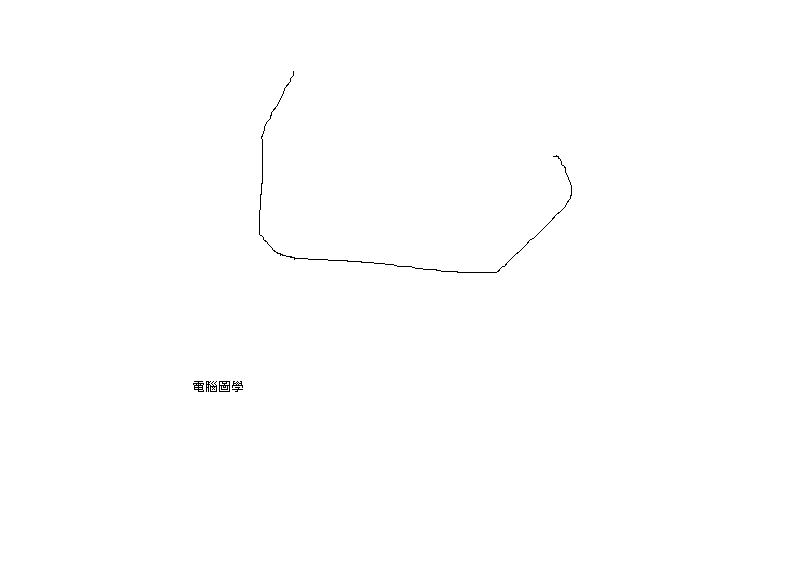
\includegraphics[width=\linewidth]{docs/figures/ch06_ppm-output.png}
        \caption{只保留 Scene 的 PPM 輸出}
        \label{fig:ppm-result}
    \end{subfigure}\hfill
    \begin{subfigure}[t]{.36\textwidth}
        \centering
        \fbox{\parbox[c][4.2cm][c]{.90\linewidth}{
                \centering 綜合繪圖成果\\
                點／鉛筆／直線／矩形／橢圓／多邊形／文字\\
                不同筆畫、填滿、接合、端點與格線
            }}
        \caption{基本工具與進階筆畫樣式}
        \label{fig:drawing-result}
    \end{subfigure}\hfill
    \begin{subfigure}[t]{.21\textwidth}
        \centering
        \fbox{\parbox[c][4.2cm][c]{.82\linewidth}{
                \centering 兩個 PaintWindow\\與確認對話框
            }}
        \caption{多視窗與確認對話框}
        \label{fig:multiwindow-result}
    \end{subfigure}
    \caption{基本繪圖與進階功能成果}
\end{figure}

\subsection{Requirement Checklist}

表~\ref{tab:requirements} 依 README 與實際程式碼標示完成狀態。介面中存在但 callback 為空，或 file command 存在但內容未序列化者，都不列為完成。

\begin{longtable}{>{\raggedright\arraybackslash}p{.24\textwidth} >{\raggedright\arraybackslash}p{.14\textwidth} >{\raggedright\arraybackslash}p{.50\textwidth}}
    \caption{作業要求與實作狀態}\label{tab:requirements}                                                                                              \\
    \toprule
    Requirement                            & Status & Implementation                                                                         \\
    \midrule
    \endfirsthead
    \toprule
    Requirement                            & Status & Implementation                                                                         \\
    \midrule
    \endhead
    Interactive 2D drawing panel           & 已完成    & CanvasElement、tool draft、Scene 與 Renderer。                                             \\
    Hierarchical menus                     & 已完成    & FreeGLUT Menu 封裝與 File/Edit/Tools/Stroke/Fill/Point/Text/Grid 子選單。                     \\
    Keyboard events                        & 已完成    & KeyDown/KeyUp/TextInput、InputState 與 ShortcutManager。                                  \\
    Mouse / motion events                  & 已完成    & MouseDown/Up/Move、Click/DoubleClick、hit test 與 mouse capture。                          \\
    Window events                          & 已完成    & Close、Reshape、Visibility、Entry callback 轉為 Window Event。                               \\
    Color                                  & 部分完成   & Stroke/Fill/Text 預設色可選；Custom color callback 尚未完成。                                     \\
    Line width / point size                & 已完成    & 選單與中括號快捷鍵可調整。                                                                          \\
    Fill mode                              & 已完成    & OUTLINE、FILLED、ADVANCED；Advanced 分開處理 Fill 與 Stroke。                                   \\
    Mouse / motion drawing                 & 已完成    & DragTool、PencilTool 與 PolygonTool。                                                     \\
    Color buffer save / restore            & 已完成    & ColorBuffer 使用 glReadPixels / glDrawPixels 做視窗 cache。                                  \\
    Save color buffer                      & 已完成    & PPM P6 export 輸出重新 render 後的 Canvas framebuffer。                                       \\
    Text input                             & 已完成    & Modal InputDialog、InputElement、TextObject 與三種字型 renderer。                              \\
    Grid                                   & 已完成    & 25 px line grid、dot grid 與 none。                                                       \\
    Grid-line / scales / positions / sizes & 部分完成   & 已有 line/dot Grid，Status Bar 會顯示游標位置與 Canvas 尺寸；程式中沒有獨立的 scale/ruler。                   \\
    Undo / Redo                            & 已完成    & CommandHistory 與 Add/Insert/Remove/Clear commands。                                     \\
    Multi-window                           & 已完成    & Application 管理視窗，Window registry 負責 callback routing；Modal Dialog 開啟時背景視窗停止接收輸入。       \\
    Save / Load document                   & 部分完成   & \lstinline|.gpt| 可寫 header/END 並有 UI/Command；Scene serialization/deserialization 尚未完成。 \\
    Selection tool                         & 已完成    & 可選取最上層圖形或文字、顯示範圍框，並以 Delete/Backspace 刪除；支援 Esc 取消與 Undo/Redo。                  \\
    PNG / JPEG export                      & 尚未完成   & 僅支援 binary PPM。                                                                        \\
    Fancy ideas                            & 已完成    & 自製 GUI、advanced stroke、GFNT、UTF-8、多視窗與 framebuffer cache。                              \\
    \bottomrule
\end{longtable}
